\documentclass[aspectratio=169]{beamer}

\makeatletter
\def\input@path{{template/}}
\makeatother

% Switch between dark and light mode:
% \usetheme[dark]{uob} (default)
% \usetheme[light]{uob}
\usetheme[dark]{uob}

\usepackage{booktabs}
\usepackage{tikz} % Added for the flowchart
\usetikzlibrary{shapes.geometric, arrows.meta, positioning}

\title{Telemetry in console systems}
\date{\today}
\author{Stan Ioan-Victor}

\begin{document}

\begin{frame}
    \titlepage
\end{frame}

\begin{frame}{About Pluton}
    \begin{quote}
        "Information is significantly harder to be removed even if an attacker installs malware or has complete physical possession of the PC." \\
        \flushright -- Microslop, talking about (personal) information, owned by those pesky hardware buyers
    \end{quote}
\end{frame}
    
\section{Telemetry concepts they all kinda use}

\begin{frame}{The big 3, and what they have in common}
        
\begin{figure}[htbp]
    \centering
    
\includegraphics[width=0.48\linewidth]{pics/noindent.png}
    \hfill
    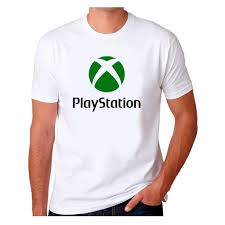
\includegraphics[width=0.48\linewidth]{pics/playbox.jpeg}
\end{figure}
    
\end{frame}

\section{What are they probing?}

\begin{frame}{What's their servers / local systems monitoring?}
    System state: 
    \begin{block}{System state:}
        Persistent logs, Hardware IDs (SoC / NAND / ROM derived ones), eFuses.
        \begin{itemize}
            \item \textbf{eFuses:} Microscopic hardware fuses blown during updates to permanently prevent firmware downgrades.
        \end{itemize}
    \end{block}

    \begin{alertblock}{Cryptography / Certification}
        Ability to sign challenges, or to decrypt info with hardware-derived private keys.
    \end{alertblock}
\end{frame}

\begin{frame}{eFuses}
    \begin{columns}[t] % [t] aligns the tops of the columns
        \begin{column}{0.48\linewidth}
            \centering
            \includegraphics[width=\linewidth]{pics/intact-efuse.jpg}
            \small\\ Intact eFuse
        \end{column}
        
        \begin{column}{0.48\linewidth}
            \centering
            \includegraphics[width=\linewidth]{pics/blown-efuse.jpg}
            \small\\ Blown eFuse
        \end{column}
    \end{columns}
\end{frame}


\section{How are they probing?}

\section{Nintendo-specific}

\begin{frame}{Nintendo: PRODINFO \& TrustZone}
    \begin{itemize}
        \item \textbf{PRODINFO Partition:} Contains the console's unique identity (hardware serial, device certificates). Banned consoles lose this "handshake" capability.
        \item \textbf{ARM TrustZone:} The Secure Processing Layer (SPL) isolated from the main HorizonOS. It handles cryptographic derivations safely out of reach from user-space.
    \end{itemize}
\end{frame}

\begin{frame}{Authentication Flow: dauth and aauth}
    \begin{center}
    \resizebox{0.9\textwidth}{!}{
    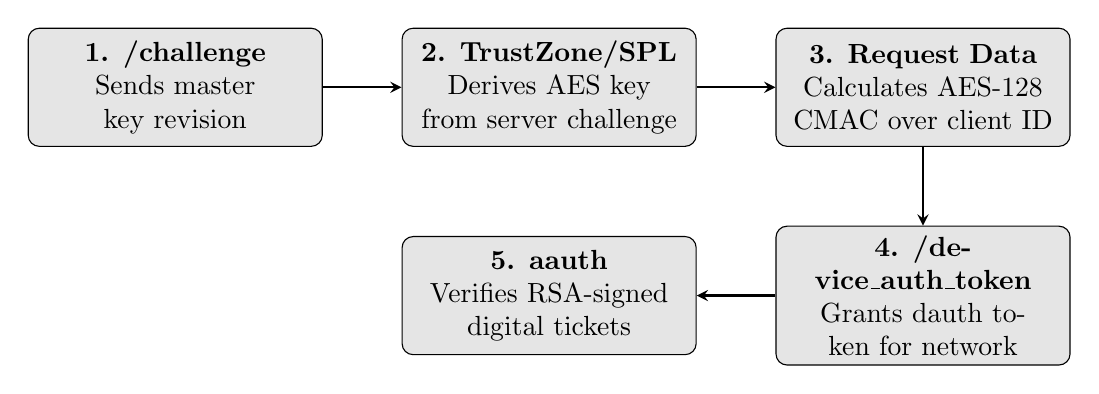
\begin{tikzpicture}[
      box/.style={rectangle, draw, fill=gray!20, text width=3.5cm, text centered, rounded corners, minimum height=1.5cm, text=black},
      arrow/.style={thick,->,>=stealth}
    ]
      \node[box] (challenge) {\textbf{1. /challenge}\\Sends master key revision};
      \node[box, right=1cm of challenge] (spl) {\textbf{2. TrustZone/SPL}\\Derives AES key from server challenge};
      \node[box, right=1cm of spl] (cmac) {\textbf{3. Request Data}\\Calculates AES-128 CMAC over client ID};
      \node[box, below=1cm of cmac] (token) {\textbf{4. /device\_auth\_token}\\Grants dauth token for network};
      \node[box, left=1cm of token] (aauth) {\textbf{5. aauth}\\Verifies RSA-signed digital tickets};

      \draw[arrow] (challenge) -- (spl);
      \draw[arrow] (spl) -- (cmac);
      \draw[arrow] (cmac) -- (token);
      \draw[arrow] (token) -- (aauth);
    \end{tikzpicture}
    }
    \end{center}
\end{frame}


\section{What the haxers did}

\begin{frame}{Those basement dwellers..}
    \begin{figure}
        \centering
        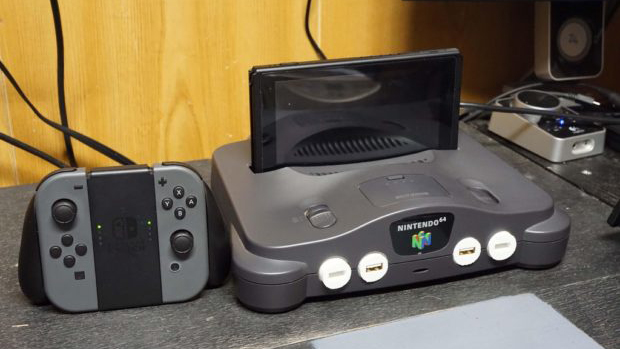
\includegraphics[width=0.4\linewidth]{pics/goofy-ahh-mod.jpg}   
        \caption{switch in NES lol}
    \end{figure}
\end{frame}

\begin{frame}{Bypass Methods: Network vs Local}
    \begin{itemize}
        \item \textbf{90DNS vs DNS MITM:}
        \begin{itemize}
            \item \textit{90DNS:} Points to an external, community-run server that blackholes Nintendo domains. Fails if you change WiFi networks.
            \item \textit{DNS MITM:} Intercepts DNS queries locally via Atmosphère and forces loopback (127.0.0.1). Much safer, system-level block.
        \end{itemize}
        \item \textbf{Exosphere vs Incognito:}
        \begin{itemize}
            \item \textit{Incognito:} Destructively overwrites the PRODINFO serial on the NAND with zeros. Dangerous if no backup exists.
            \item \textit{Exosphere:} Spoofs the serial number in memory (TrustZone/EL3 level). Leaves physical NAND untouched.
        \end{itemize}
    \end{itemize}
\end{frame}

\section{Xbox-specific}

\begin{frame}{Xbox: Pluton \& The Death of the Bus}
    \begin{itemize}
        \item \textbf{The Old Flaw:} Discrete TPMs sent decryption keys (like BitLocker keys) over the motherboard's LPC/SPI bus. Attackers physically snooped the bus to steal secrets. You couldn't fake the signature, but you could steal the data in transit.
        \item \textbf{The Pluton Fix:} Integrated directly into the CPU silicon. No external communication bus exists to sniff.
        \item \textbf{Measurements \& Tokens:} During boot, Pluton takes "measurements" (SHA-256 hashes) of the UEFI and kernel. The server verifies these hashes before granting an authorization token for Xbox Live. It's for network access, not per-instruction CPU execution.
    \end{itemize}
\end{frame}

\section{What the haxers did}

\begin{frame}{Can Xbox even be bypassed?}
    \begin{itemize}
        \item Short answer: Not easily. It is highly resilient to traditional bypassing.
        \item \textbf{Dev Mode:} Microsoft provides an official "Dev Mode" that allows sideloading UWP apps (like emulators). This ironically acts as a pressure valve, reducing the community incentive to hunt for deep hypervisor exploits.
        \item \textbf{Hypervisor Isolation:} The SystemOS and Game (ERA) partitions are strictly separated. Escaping the game container to access the core system requires defeating enterprise-grade Hyper-V boundaries.
    \end{itemize}
\end{frame}

\section{BlaySteition-specific}

\begin{frame}{Baby Station (PS4/PS5)}
    \begin{itemize}
        \item \textbf{Encrypted Filesystems:} Relies on a non-standard, heavily encrypted FreeBSD-based filesystem.
        \item Telemetry modifications are exceptionally difficult, so evasion focuses on network blocking and maintaining exploitability.
    \end{itemize}
\end{frame}

\section{What the haxers did}

\begin{frame}{PlayStation: Update Blockers \& Fake Sign-ins}
    \begin{itemize}
        \item \textbf{Maintaining Exploitable Firmware:} Bypassing telemetry relies on not updating.
        \item \textbf{The Directory Trick:} Creating folders named \texttt{PS4UPDATE.PUP} and \texttt{PS4UPDATE.PUP.TEMP}. Because a directory cannot be overwritten by a file with the exact same name, the console is physically unable to download the update package.
        \item \textbf{Fake Sign-in:} Bypassing the heartbeat signals to the PlayStation Network (PSN) while keeping local network features active for homebrew.
    \end{itemize}
\end{frame}

\end{document}
